%% 電子情報工学演習 セミナー資料 RC-03
%% 可逆プログラムは何を払っているか（Janus 系コーパス111本の資源アトラス）
%% Build: make rc03（platex -> dvipdfmx）
\documentclass[a4paper,11pt]{jsarticle}
\usepackage{amsmath,amssymb}
\usepackage[dvipdfmx]{graphicx}
\usepackage{booktabs}
\usepackage{url}
\usepackage[dvipdfmx,hidelinks]{hyperref}
\def\UrlBreaks{\do\/\do-\do.\do:}
\Urlmuskip=0mu plus 3mu
\emergencystretch=1em
\setlength{\parskip}{2pt}

\newcommand{\Mstar}{\ensuremath{M^{*}}}
\newcommand{\pmin}{\ensuremath{p_{\min}}}

\title{可逆プログラムは何を払っているか\\
\large Janus 系コーパス 111 本の資源アトラス\\
\large 電子情報工学演習 セミナー資料 RC-03}
\author{横山 哲郎（南山大学 理工学部 電子情報工学科）}
\date{2026 年 8 月 30 日 12 時 16 分（JST）作成\\版 1.0}

\begin{document}
\maketitle

\section*{この文書について}
本資料は電子情報工学演習のセミナー資料である．査読を受けた論文ではなく，
ゼミで読むための解説として書いた．結果はすべて機械実験であり，定理は主張しない．
本資料の版は \url{https://github.com/tetsuo-jp/rc-lecture-notes} にある．

\section*{概要}
可逆プログラミング言語は不可逆な消去を禁じる．では計算の代価はどこへ移るのか．
本資料は Janus 系のコーパス 111 本について，生存状態・スタック・時間を同時に実測し，
区分ごとに見渡せる形に整理した資源アトラスを与える．
消去が使われないだけでなく，中間結果も片づけられない．
書き込みのあった配列の約 65\% は値を 0 に戻す操作を一度も持たず，
終端で空になる配列は約 13\% にとどまる．
規模とともに増える代価はスタックであり，
その主な消費者は再帰的なメモ化に限らずグラフ探索と平衡木の操作である．
動的計画法の族についてはクリーンな可逆ペブリングの厳密最適を基準線として添え，
クリーン性を捨てる利得と代価を即値で示す．

\section{まえがき}\label{sec:intro}

可逆プログラミング言語は，各文が単射な状態変換を表すことを構文の段階で保証し，
値を捨てる代入や制御の合流を禁じる\cite{LRR82:janus,GlYo23:perspective}．
この制約は，情報の消去に物理的な代価が伴うという指摘\cite{Land91}と，
消去を使わずに計算を実現できるという結果\cite{Benn73}に由来する．
ここから素朴な期待が生じる．すなわち，可逆プログラムは何も捨てないのだから，
計算が終わったときに余分なものを残さない，という期待である．
しかし消去を禁じても計算が安くなるわけではない．代価は消える先を失って，
どこか別の資源へ移るはずである．本資料はこの移り先を実測で特定する．

払われる資源の理論的な扱いは，可逆ペブリング遊戯として整備されてきた．
消去を許さない模型では領域と時間の交換関係が厳密に解析され\cite{LiTV98}，
量子コンパイルの補助量子ビット割当てにも応用されている\cite{Meuli19:pebbling}．
言語側でも，可逆メモ化のように個々のプログラムの資源使用を解析した研究がある\cite{Yoko17}．
ただし前者が対象とするのは依存グラフという抽象であり，後者が扱うのは少数のプログラムである．
実在の可逆プログラムがどの資源をどれだけ払っているかを，コーパスの規模で横断的に
測った報告は，著者の知る限り無い．

本資料は Janus 系のコーパス 111 本を対象に，生存状態・スタック・時間の 3 資源を
同時に実測し，区分ごとに見渡せる形に整理した資源アトラスを与える．寄与は 3 点である．
第一に，消去が使われないだけでなく，中間結果も片づけられない．
書き込みのあった配列の約 65\% は一度も値を 0 に戻さず，
終端で空になる配列は約 13\% にとどまる（\ref{sec:census}節）．
第二に，規模とともに増える代価はスタックであり，その主な消費者は再帰的なメモ化に限らず，
グラフ探索と平衡木の操作である（\ref{sec:census}節，\ref{sec:scaling}節）．
第三に，依存グラフを取り出せる動的計画法の族については，クリーンな可逆ペブリングの
厳密最適を基準線として添え，クリーン性を捨てる利得と代価を即値で示す（\ref{sec:baseline}節）．
本資料の結果はすべて機械実験であり，定理は主張しない．

\section{対象と計測法}\label{sec:method}

本資料が対象とするのは，Janus 系の可逆プログラム 111 本である\cite{LRR82:janus}．
内訳は，整列・グラフ・動的計画法・圧縮・単射関数・構造体の各領域にわたる
PyJanus\footnote{Janus の Python 処理系．\url{https://github.com/yokoyama-lab/PyJanus}}
のフィクスチャ 97 本，jana の例題 7 本，可逆メモ化の実装 7 本である\cite{Yoko17}．
母数 120 本のうち 9 本は対象から外した．8 本は方言の差により構文解析に至らず，
1 本は局所変数の解放時の表明に失敗して実行時に停止したためである．
除外したものも実行センサスに記録を残し，成功率そのものを処理系の方言被覆率として報告する．
なお PyJanus のフィクスチャはコミット \texttt{c6c1656} 時点の 97 本である．
その後フィクスチャは全件が改名されて 101 本になっており，
本資料の 111 本を再現するにはこのコミットを指定する必要がある．

各プログラムに対して，表\ref{tab:metrics}の資源ベクトルを記録する．
時間の代理には実行文数 $\mathit{steps}$ を用い，空間は 2 種に分けて測る．
すなわち，呼び出し時に退避される値の総深さのピーク $\mathit{stack\_peak}$ と，
終端で 0 でない状態の量 $\mathit{final\_live\_bits}$ である．
配列については，値を 0 から非 0 にする操作と，その逆の操作を配列ごとに数える．
判定できない量は空欄とし，推定では埋めない．
とくに $\mathit{final\_live\_bits}$ は値として報告するにとどめ，
終端の状態が不要なゴミか出力かの判定はしない．
Janus では終端の記憶域全体が出力であり，どの変数が出力かは注釈なしには決まらないためである．

\begin{table}[tb]
  \centering
  \caption{1 プログラムにつき記録する資源ベクトル．$\mathit{erasures}$ は
    言語が不可逆消去を禁じるため恒等的に 0 であり，測るまでもなく 0 であること自体が
    本資料の出発点である．}
  \label{tab:metrics}
  \small
  \setlength{\tabcolsep}{3pt}
  \begin{tabular}{l l}
    \toprule
    量 & 定義 \\
    \midrule
    $\mathit{steps}$ & 実行した文の数（時間の代理） \\
    $\mathit{stack\_peak}$ & 全フレームの退避値の総深さのピーク \\
    $\mathit{call\_depth\_peak}$ & 呼び出しの深さのピーク \\
    $\mathit{final\_live\_bits}$ & 終端で 0 でない状態のビット数 \\
    $\mathit{puts}$ / $\mathit{takes}$ & 配列セルの $0 \to$ 非 $0$ と逆向きの回数 \\
    $\mathit{erasures}$ & 不可逆な消去の回数（恒等的に 0） \\
    \bottomrule
  \end{tabular}
\end{table}

計測器は，1 文ごとに記憶域の状態を走査する解釈器の計装として実装した．
参照で渡された配列を重複して数えないよう，記憶域のセルは同一性で識別する．
妥当性は 3 通りの照合で担保した．
第一に，本研究の予備実験で個別に測定済みであった 5 本の値を回帰試験に固定した．
第二に，素朴な実装と高速な実装を独立に書き，重なる範囲での一致を確認した．
第三に，実行文数を処理系に付属する既存のプロファイラと突き合わせた．
この照合は実際に誤りを 1 件検出した．予備実験でスタックのピークを $75{,}802$ と
記録していた実装について，正しい値は $310$ であり，
差は参照で渡されたセルを重複して数えたことによるものであった．
この 2 実装の照合はのちに \ref{sec:census}節の別コーパスを含む 219 本へ広げ，
共通の定義を持つ $\mathit{steps}$ と $\mathit{call\_depth\_peak}$ について
219 本すべてで一致することを確かめた．
また，フィクスチャの改名をまたいだ再計測でも，改名の記録から対応づけた 97 本すべてで
資源ベクトルの 4 つの値が一致した．

\section{全数計測}\label{sec:census}

111 本すべてを固定入力で実行し，資源ベクトルを得た（表\ref{tab:category}）．
$\mathit{steps}$ の中央値は 74，最大は $27{,}157$ であり，
これは棒の切り出し問題（cut rod）でメモ表を 2 つ持つ実装である．
$\mathit{stack\_peak}$ は中央値が 0，最大が 310（切り出し問題の上向き再帰の実装）であり，
$\mathit{final\_live\_bits}$ は中央値 21，最大 343（全点対最短路の実装）であった．
中央値の段階でスタックが 0 であることは，
コーパスの半数以上が値の退避を一度も必要としないことを意味する．

このコーパスから 2 つの事実が読める．第一は，消去についてである．
$\mathit{erasures}$ は 111 本すべてで 0 であった．これは言語が消去を禁じる以上，
測るまでもない．終端で状態がすべて 0 になるプログラムもまた 0 本であったが，
Janus では終端の記憶域全体が出力であるから，これも言語の定義から予想される．
問うべきは，補助的に使われた記憶が片づけられるかである．
配列の水準で見ると，書き込みのあった 189 本の配列のうち 122 本（約 $65\%$）は
値を 0 に戻す操作を一度も行わず，終端で空になる配列は 25 本（約 $13\%$）にとどまる．
すなわち本コーパスの典型的な可逆プログラムは，逆計算によって中間結果を片づけることをせず，
結果と中間物の両方を記憶域に残したまま終了する．
計算が終われば余分なものは残らない，という\ref{sec:intro}節の素朴な期待は，
配列の水準で見ても 3 本に 2 本の割合で裏切られる．

第二は，払われている資源の所在である．
スタックを使うのは 111 本中 36 本であり，使用量の上位は
切り出し問題の上向き再帰（310），AVL 木の削除（79），全点対最短路（67），
AVL 木の挿入（65），強連結成分分解（60），単一始点最短路（54）である．
すなわちスタックの主要な消費者は，再帰的なメモ化に限らず，
グラフ探索と平衡木の操作である．
一方で単射関数の実装は 15 本中 1 本，構造体の操作は 13 本中 0 本しかスタックを使わない．
資源の消費は領域によって偏っており，「スタック支配型」と呼べる区分が実在する．
ただし構造体の区分は言語機能の試験を含み，実行文数の中央値が 7 と小さい．
この区分についてはプログラムの小ささが効いている可能性を排除できない．
図\ref{fig:scatter}はこの偏りを示す．横軸に実行文数，縦軸にスタックのピークを取ると，
スタックを使わない 75 本が底の帯に並び，その上に離れてアルゴリズムとメモ化が分布する．

以上の割合が本コーパスに固有のものかを確かめるため，収集の目的が異なる別のコーパスに
同じ計測器を当てた．アルゴリズムを集めることを目的として別に整備された可逆アルゴリズム集
118 本である．こちらでは $\mathit{stack\_peak}$ が正のものが 118 本中 69 本（約 $58\%$）あり，
中央値も 0 ではなく 6 であった．
代価がスタックへ移るという観察は，アルゴリズムを目的に集めたコーパスでこそ強く出る．
逆に言えば，本節の $32\%$（111 本中 36 本）は母集団に依存する量であり，
どの母集団を測った値かと切り離しては読めない（\ref{sec:conclusion}節）．
一方，配列についての 2 つの観察は母集団を変えても保たれた．
終端で状態がすべて 0 になるプログラムは，この 118 本と改名後の PyJanus のフィクスチャ
101 本を合わせた 219 本のいずれにも無い．
値を 0 に戻す操作を持たない配列は，書き込みのあった配列のうち約 $59\%$（240 本中 141 本）と
約 $68\%$（177 本中 121 本）であり，終端で空になる配列は約 $10\%$（240 本中 25 本）と
約 $13\%$（177 本中 23 本）であった．

\begin{figure}[tb]
  \centering
  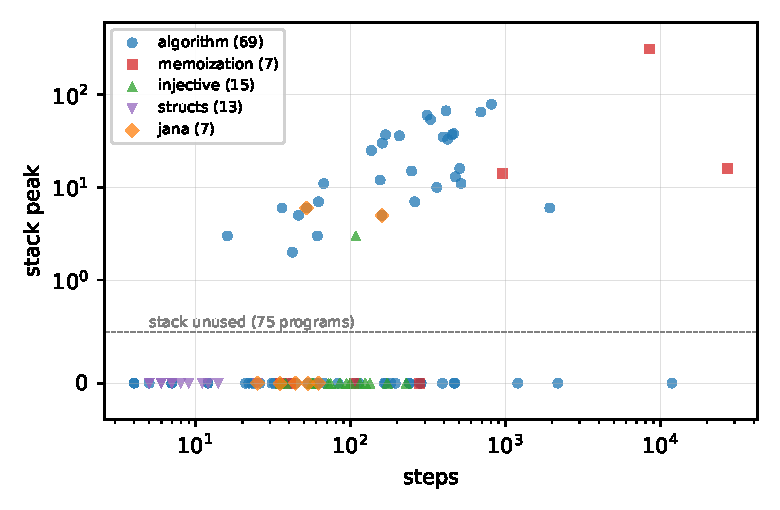
\includegraphics[width=\linewidth]{assets/figs/fig1_stack_vs_steps.pdf}
  \caption{111 本の $\mathit{steps}$ と $\mathit{stack\_peak}$．縦軸は 0 を含めるため
    原点付近を線形にした対数軸である．破線より下の帯はスタックを使わない 75 本であり，
    構造体と単射関数の実装はほぼこの帯に属する．}
  \label{fig:scatter}
\end{figure}

\begin{table}[t]
  \centering
  \caption{区分ごとの要約（111 本）．スタックを使う本数は
    $\mathit{stack\_peak}>0$ の本数である．}
  \label{tab:category}
  \small
  % 自動生成（scripts/gen_atlas_tables.py）。手編集しないこと。
\begin{tabular}{l r r r r}
\toprule
区分 & 本数 & steps 中央値 & スタックを使う本数 & $\mathit{final\_live\_bits}$ 中央値 \\
\midrule
アルゴリズム & 69 & 159 & 30/69 & 26 \\
メモ化 & 7 & 279 & 3/7 & 46 \\
単射関数 & 15 & 94 & 1/15 & 19 \\
構造体 & 13 & 7 & 0/13 & 17 \\
jana & 7 & 52 & 2/7 & 9 \\
\bottomrule
\end{tabular}

\end{table}

\section{規模を振った計測}\label{sec:scaling}

固定入力の計測は規模の比較を与えない．そこで入力の大きさを変えられる 9 族について，
各 6 つの大きさで測り直した（54 点，表\ref{tab:scaling}）．
入力は縮小版と拡大版を別に用意し，コーパスの原本は改変していない．
成長の速さについては，実測列と隣接する 2 点の比のみを報告し，閉じた式の当てはめはしない．
少数の点への当てはめは本研究の予備実験でも繰り返し崩れており，
6 点程度で漸近の主張をしないことを方針とした．

隣接比の推移から，9 族は 3 つの群に分かれる．
線形群では一階差分が 6 点すべてで一定であり，反復版のフィボナッチ（差分 20），
最大公約数（差分 8），そして隣り合う 2 項を対で持ち回るフィボナッチのメモ化
（以下，対のメモ化．差分 7）がここに入る．
対のメモ化は可逆メモ化の実装であり，\ref{sec:baseline}節の基準線でも中心的な例となる．
多項式群では隣接比が 1 に向かって単調に減少し，バブルソートと
3 つの動的計画法（編集距離，最長共通部分列，ナップサック）が該当する．
急成長群では隣接比が定数に張り付き，階乗の実装は 4.00 に，
切り出し問題の実装は 2.27 に近づく．
規模を振った 9 族の中では，再帰の逆計算を素朴に書いた階乗の実装が最も高くつく．
図\ref{fig:ratios}に隣接比の推移を示す．3 群は線種で分けており，
群の分かれは末端の比だけで判定できる．

規模を振ると，スタックの増え方が族ごとに読める．
引数をフィボナッチ数とした最大公約数の族では，除算の回数 $k$ とスタックのピークが
6 点すべてで一致した．バブルソートでは比較の回数 $n(n-1)/2$ と一致し，
切り出し問題の実装では $\mathit{stack\_peak}/\mathit{steps}$ が
6 点すべてで 0.104 から 0.112 の範囲に収まる．
最後の観察は，可逆メモ化の実装では記憶量が実行時間に比例するという
先行研究の指摘\cite{Yoko17}を，規模を振った実測として裏づけるものである．
一方，上向きの動的計画法 3 族はどの大きさでもスタックを使わない．
上向きの動的計画法がスタックを使わないという\ref{sec:census}節の観察は，
規模を変えても保たれる．ただし規模を振った 9 族にはグラフ探索と平衡木の実装が
含まれないため，それらの区分については規模を変えた確認をしていない．
なお，これらの等式は 6 点での一致であって証明ではない．

\begin{figure}[tb]
  \centering
  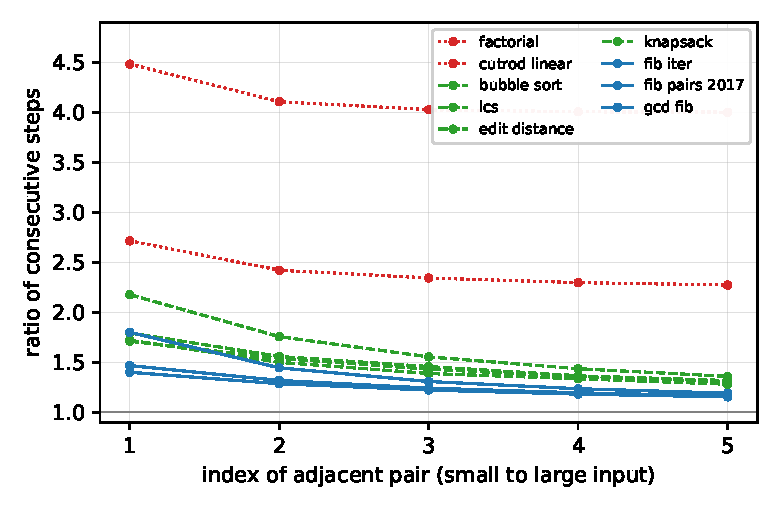
\includegraphics[width=\linewidth]{assets/figs/fig2_ratios.pdf}
  \caption{9 族の隣接比の推移．横軸は小さい入力から順に並べた隣接する 2 点の組であり，
    線種は成長の 3 群（点線は急成長群，破線は多項式群，実線は線形群）に対応する．
    群の分かれは末端の比で判定でき，境界に乗る族は無い．}
  \label{fig:ratios}
\end{figure}

\begin{table}[t]
  \centering
  \caption{9 族を 6 サイズで測った結果．当てはめはせず，実測列と隣接比のみを示す．
    $\mathit{stack\_peak}$ の 0 は全点で 0 であることを表す．}
  \label{tab:scaling}
  \small
  % 自動生成（scripts/gen_atlas_tables.py）。手編集しないこと。
\begin{tabular}{l l c c}
\toprule
族 & steps（6 点） & 隣接比（初 $\to$ 末） & $\mathit{stack\_peak}$ \\
\midrule
fib\_iter & 25, 45, 65, 85, 105, 125 & 1.80 $\to$ 1.19 & 0 \\
factorial & 31, 139, 571, 2299, 9211, 36859 & 4.48 $\to$ 4.00 & 0 \\
gcd\_fib & 20, 28, 36, 44, 52, 60 & 1.40 $\to$ 1.15 & 4 $\to$ 14 \\
bubble\_sort & 68, 148, 260, 404, 580, 788 & 2.18 $\to$ 1.36 & 6 $\to$ 91 \\
edit\_distance & 52, 89, 137, 196, 266, 347 & 1.71 $\to$ 1.30 & 0 \\
lcs & 29, 52, 81, 118, 161, 212 & 1.79 $\to$ 1.32 & 0 \\
knapsack & 50, 86, 129, 179, 239, 306 & 1.72 $\to$ 1.28 & 0 \\
fib\_pairs & 15, 22, 29, 36, 43, 50 & 1.47 $\to$ 1.16 & 0 \\
cutrod\_linear & 210, 570, 1380, 3234, 7428, 16878 & 2.71 $\to$ 2.27 & 22 $\to$ 1874 \\
\bottomrule
\end{tabular}

\end{table}

\section{厳密最適の基準線}\label{sec:baseline}

\begin{table}[t]
  \centering
  \caption{基準線が届いた最大サイズの 1 行（族ごと）．$N$ は依存 DAG の節点数であり，
    目標の値に寄与しない節点は含めない．
    \Mstar と \pmin はクリーンな可逆ペブリングの厳密最適である．
    $\dagger$ は impl peak $<$ \pmin であり，モデル対応が成立しないことを表す
    （\ref{sec:baseline}節）．}
  \label{tab:baselines}
  \small
  % 自動生成（scripts/gen_atlas_tables.py）。手編集しないこと。
\begin{tabular}{l r r r r r r r}
\toprule
族 & $n$ & $N$ & 床 $2N-1$ & $M^{*}$ & $p_{\min}$ & 実装の手数 & 実装のピーク \\
\midrule
fib\_pairs & 13 & 7 & 13 & 19 & 4 & 7 & 7 \\
edit\_distance & 5 & 25 & 49 & 117 & 10 & 35 & 35 \\
lcs & 5 & 25 & 49 & 117 & 10 & 24 & 24 \\
knapsack & 5 & 22 & 43 & 103 & 7 & 33 & 33 \\
cutrod\_linear $\dagger$ & 14 & 14 & 27 & 27 & 14 & 1246 & 10 \\
\bottomrule
\end{tabular}

\end{table}

実測値だけでは，払っている量が多いのか少ないのかを判断できない．
そこで依存グラフを取り出せる族に限り，クリーンな可逆ペブリングの厳密最適を
基準線として添えた（表\ref{tab:baselines}）．
ここでクリーンとは，計算の終了時に入力と出力以外のペブルをすべて取り除いた状態を指し，
手数とはペブルを置く操作と取り除く操作の総数である．
対象は動的計画法の 5 族であり，各族の依存グラフに対して，
最小の同時保持数 \pmin と，その下での最小手数 \Mstar を，
状態空間の双方向幅優先探索と制約充足ソルバの併用によって厳密に決めた．
節点数が 25 を超える大きさは探索が届かないため空欄とし，推定値では埋めない．
コーパス全体に基準線を付けることはできない．
依存グラフの取り出し方が定義できないプログラムが大半だからである．

基準線を添えると，クリーン性を捨てることの意味が即値になる．
対のメモ化の $n=13$ では，実装の手数は 7 であり，
クリーンな計算に必要な手数の下限 $2N-1=13$ を下回る．
すなわち実装は，クリーン性を捨てることで，いかなるクリーンな計画よりも速い．
その代価は，全節点を保持するピーク（この例では 7）と，終端に残る中間結果である．
逆に，同じ計算をクリーンに行う費用も即値で読める．
編集距離の $n=5$ では，手数は 35 から 117 へ 3.3 倍になる一方，
同時保持数は 35 から 10 へ 3.5 分の 1 になる．
なお編集距離と最長共通部分列は同一の依存グラフを持ち基準線も一致するが，
実装の手数は 35 と 24 で異なる．境界の初期化の差であり，
模型が同じでも実装の定数は異なることを示している．

この照合は，最適性の尺度としてだけでなく，模型の対応付けの検査としても働いた．
切り出し問題の族では，実装のピークが 10 であるのに \pmin が 14 と算出された．
同時保持数の最小値を下回る実行は存在しえないため，これは対応付けの誤りを意味する．
原因は依存関係の取り方にあった．全履歴を残す依存グラフは，
ある値を置くときにそれ以前のすべての値が同時に必要であるとするが，
実装は最大値を逐次に累積するので，過去の値を一つずつ使って消費する．
同時可用性を要求するペブリングの前提が，この族の実装には当てはまらない．
したがって表\ref{tab:baselines}の当該行は無効として扱い，印を付けて残した．
他の 4 族では実装のピークが \pmin 以上であり，対応付けの妥当性が同じ照合で裏づけられた．

\section{限界とまとめ}\label{sec:conclusion}

本資料の結果には次の限界がある．
第一に，計測の大半は固定入力によるものであり，規模を振ったのは 9 族に限られる．
第二に，終端に残る状態は量として報告するのみで，
それが出力かゴミかの判定はしていない（\ref{sec:method}節）．
第三に，基準線は節点数 25 以下の大きさにしか届かず，
切り出し問題の族については模型の対応付け自体が成立しない（\ref{sec:baseline}節）．
第四に，方言の差により 8 本，実行時の表明の失敗により 1 本を対象から外しており，
被覆は処理系に依存する．
第五に，\ref{sec:scaling}節のスタックの等式は 6 点での一致であって証明ではない．
第六に，本資料の割合は母集団に依存する．本コーパスの主要部は処理系のフィクスチャであり，
スタックを使う本数の割合は 111 本中 36 本（約 $32\%$）であるのに対し，
アルゴリズムを目的に集めたコーパスでは 118 本中 69 本（約 $58\%$）である
（\ref{sec:census}節）．割合を引用するときは，どのコーパスの何本かを添える必要がある．
本資料の主張はいずれも機械実験の水準にとどまり，定理としては述べていない．

本資料は，Janus 系のコーパス 111 本について，生存状態・スタック・時間を同時に実測した
資源アトラスを与えた．消去が使われないだけでなく中間結果も片づけられず，
書き込みのあった配列の約 $65\%$ は値を戻す操作を持たず，
終端で空になる配列は約 $13\%$ にとどまる．
この 2 つは，別に整備されたコーパスを含む 219 本でも同じ向きに再現した．
規模とともに増える代価はスタックであり，その主な消費者はグラフ探索と平衡木の操作である．
動的計画法の族では，クリーン性を捨てることが手数を下限より小さくする一方，
同じ計算をクリーンに行えば手数は 3.3 倍になり同時保持数は 3.5 分の 1 になる．
計測器・入力・表と図の生成手順はすべて公開し，乱数を使わない決定的な実行として構成した．
同じ入力からは同じ表と図が再生成される．

\begin{thebibliography}{9}
\bibitem{LRR82:janus} C. Lutz and H. Derby, ``Janus: a time-reversible language,''
Letter to R. Landauer, 1982.
\bibitem{GlYo23:perspective} R. Gl\"uck and T. Yokoyama, ``Reversible computing from a
programming language perspective,'' Theoretical Computer Science, vol.953, p.113429, 2023.
\bibitem{Land91} R. Landauer, ``Information is physical,'' Physics Today, vol.44, no.5,
pp.23--29, 1991.
\bibitem{Benn73} C.H. Bennett, ``Logical reversibility of computation,''
IBM J. Res. Dev., vol.17, no.6, pp.525--532, 1973.
\bibitem{LiTV98} M. Li, J. Tromp, and P. Vit\'anyi, ``Reversible simulation of
irreversible computation,'' Physica D, vol.120, no.1-2, pp.168--176, 1998.
\bibitem{Meuli19:pebbling} G. Meuli, M. Soeken, M. Roetteler, N. Bjorner, and
G. De Micheli, ``Reversible pebbling game for quantum memory management,''
Design, Automation and Test in Europe (DATE), pp.288--291, 2019.
\bibitem{Yoko17} 横山哲郎, ``可逆プログラムのための償却定数時間・定数ゴミのメモ化,''
vol.J100-D, no.10, pp.895--896, 2017.
\end{thebibliography}

\end{document}
